% Shared standalone design for the editable figure reconstructions.
\documentclass[tikz,border=5pt,10pt]{standalone}
\usepackage[T1]{fontenc}
\usepackage[utf8]{inputenc}
\usepackage{newpxtext,newpxmath}
\usepackage[scaled=.94]{sourcesanspro}
\usepackage{pgfplots}
\pgfplotsset{compat=1.18}
\usetikzlibrary{arrows.meta,calc,positioning,decorations.pathreplacing,
  decorations.markings,patterns,matrix,shapes.geometric,fit,backgrounds,
  intersections,angles,quotes}
\definecolor{ink}{HTML}{203746}
\definecolor{accent}{HTML}{146C78}
\definecolor{muted}{HTML}{667780}
\definecolor{signalred}{HTML}{B94B44}
\color{ink}
\tikzset{>=Latex,line width=.8pt,
  every node/.style={font=\small},
  axis/.style={->,draw=muted,line width=.5pt},
  guide/.style={draw=muted,dashed,line width=.45pt},
  curve/.style={draw=accent,line width=1pt},
  marker/.style={circle,fill=accent,inner sep=1.5pt},
  labelbox/.style={fill=white,inner sep=2pt}}

\begin{document}
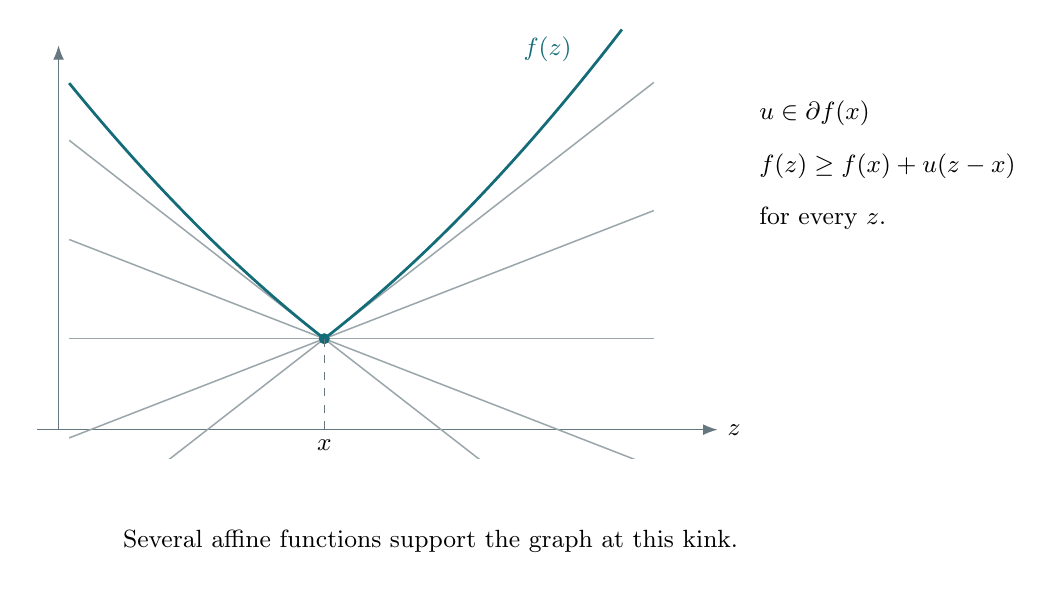
\begin{tikzpicture}[x=1.35cm,y=1.05cm]
\draw[axis](-2.7,0)--(3.7,0)node[right]{$z$};\draw[axis](-2.5,0)--(-2.5,4.65);
\begin{scope}\clip(-2.5,-.35)rectangle(3.2,4.8);\foreach \u in {-1,-.5,0,.5,1}{\draw[muted!65,line width=.55pt](-2.4,{1.1-2.4*\u})--(3.1,{1.1+3.1*\u});}
\end{scope}\draw[curve]plot[domain=-2.4:0,samples=40](\x,{1.1-\x+.12*\x*\x});
\draw[curve]plot[domain=0:2.8,samples=40](\x,{1.1+\x+.12*\x*\x});
\fill[accent](0,1.1)circle(2pt);\draw[guide](0,0)node[below]{$x$}--(0,1.1);
\node[accent]at(2.1,4.6){$f(z)$};
\node[anchor=west,align=left]at(4.0,3.2){$u\in\partial f(x)$\\[8pt]$f(z)\geq f(x)+u(z-x)$\\[8pt]for every $z$.};
\node[align=center,text width=10cm]at(1,-1.35){Several affine functions support the graph at this kink.};
\end{tikzpicture}
\end{document}
